% DPF 09 talk on strangeness in nucleon

\documentclass[10pt]{beamer}
\usepackage{amsmath}
\usepackage{mathtools}
\usefonttheme{professionalfonts} % using non standard fonts for beamer
\usefonttheme{serif} % default family is serif


%\documentclass[12pt]{beamerthemeSam.sty}
\usepackage{epsf}
%\usepackage{pstricks}
%\usepackage[orientation=portrait,size=A4]{beamerposter}
\geometry{paperwidth=160mm,paperheight=120mm}
%DT favorite definitions
\def\LL{\left\langle}	% left angle bracket
\def\RR{\right\rangle}	% right angle bracket
\def\LP{\left(}		% left parenthesis
\def\RP{\right)}	% right parenthesis
\def\LB{\left\{}	% left curly bracket
\def\RB{\right\}}	% right curly bracket
\def\PAR#1#2{ {{\partial #1}\over{\partial #2}} }
\def\PARTWO#1#2{ {{\partial^2 #1}\over{\partial #2}^2} }
\def\PARTWOMIX#1#2#3{ {{\partial^2 #1}\over{\partial #2 \partial #3}} }

\def\rightpartial{{\overrightarrow\partial}}
\def\leftpartial{{\overleftarrow\partial}}
\def\diffpartial{\buildrel\leftrightarrow\over\partial}

\def\BI{\begin{itemize}}
\def\EI{\end{itemize}}
\def\BE{\begin{displaymath}}
\def\EE{\end{displaymath}}
\def\BEA{\begin{eqnarray*}}
\def\EEA{\end{eqnarray*}}
\def\BNEA{\begin{eqnarray}}
\def\ENEA{\end{eqnarray}}
\def\EL{\nonumber\\}
\definecolor{A}{rgb}{0.8,0.0,0.0}
\definecolor{B}{rgb}{0.0,0.6,0.0}
\definecolor{C}{rgb}{0.6,0.6,0.0}
\definecolor{D}{rgb}{0.0,0.0,0.5}
\definecolor{E}{rgb}{0.4,0.4,0.4}

\newcommand{\map}[1]{\frame{\frametitle{\textbf{Course map}}
\centerline{\includegraphics[height=0.86\paperheight]{../../map/#1.png}}}}
\newcommand{\wmap}[1]{\frame{\frametitle{\textbf{Course map}}
\centerline{\includegraphics[width=0.96\paperwidth]{../../map/#1.png}}}}

\newcommand{\etal}{{\it et al.}}
\newcommand{\gbeta}{6/g^2}
\newcommand{\la}[1]{\label{#1}}
\newcommand{\ie}{{\em i.e.\ }}
\newcommand{\eg}{{\em e.\,g.\ }}
\newcommand{\cf}{cf.\ }
\newcommand{\etc}{etc.\ }
\newcommand{\atantwo}{{\rm atan2}}
\newcommand{\Tr}{{\rm Tr}}
\newcommand{\dt}{\Delta t}
\newcommand{\op}{{\cal O}}
\newcommand{\msbar}{{\overline{\rm MS}}}
\def\chpt{\raise0.4ex\hbox{$\chi$}PT}
\def\schpt{S\raise0.4ex\hbox{$\chi$}PT}
\def\MeV{{\rm Me\!V}}
\def\GeV{{\rm Ge\!V}}

%AB: my color definitions
%\definecolor{mygarnet}{rgb}{0.445,0.184,0.215}
%\definecolor{mygold}{rgb}{0.848,0.848,0.098}
%\definecolor{myg2g}{rgb}{0.647,0.316,0.157}
\definecolor{abtitlecolor}{rgb}{0.0,0.255,0.494}
\definecolor{absecondarycolor}{rgb}{0.0,0.416,0.804}
\definecolor{abprimarycolor}{rgb}{1.0,0.686,0.0}
\definecolor{Red}           {cmyk}{0,1,1,0}
\definecolor{Grey}           {cmyk}{.7,.7,.7,0}
\definecolor{Blue}          {cmyk}{1,1,0,0}
\definecolor{Green}         {cmyk}{1,0,1,0}
\definecolor{Brown}         {cmyk}{0,0.81,1,0.60}
\definecolor{Black}         {cmyk}{0,0,0,1}

\usetheme{Madrid}


%AB: redefinition of beamer colors
%\setbeamercolor{palette tertiary}{fg=white,bg=mygarnet}
%\setbeamercolor{palette secondary}{fg=white,bg=myg2g}
%\setbeamercolor{palette primary}{fg=black,bg=mygold}
\setbeamercolor{title}{fg=abtitlecolor}
\setbeamercolor{frametitle}{fg=abtitlecolor}
\setbeamercolor{palette tertiary}{fg=white,bg=abtitlecolor}
\setbeamercolor{palette secondary}{fg=white,bg=absecondarycolor}
\setbeamercolor{palette primary}{fg=black,bg=abprimarycolor}
\setbeamercolor{structure}{fg=abtitlecolor}

\setbeamerfont{section in toc}{series=\bfseries}

%AB: remove navigation icons
\beamertemplatenavigationsymbolsempty
\title[Vectors and 2D kinematics]{
  \textbf {Vectors and 2D kinematics}\\
%\centerline{}
%\centering
%\vspace{-0.0in}
%\includegraphics[width=0.3\textwidth]{propvalues_0093.pdf}
%\vspace{-0.3in}\\
%\label{intrograph}
}

\author[W. Freeman] {Physics 211\\Syracuse University, Physics 211 Spring 2022\\Walter Freeman}

\date{\today}

\begin{document}

\frame{\titlepage}

\frame{\frametitle{\textbf{ }}
\large

``Poets say science takes away from the beauty of the stars -- mere globs of gas atoms. Nothing is “mere.” I too can see the stars on a desert night, and feel them. But do I see less or more? The vastness of the heavens stretches my imagination--stuck on this carousel my little eye can catch one-million-year-old light. A vast pattern, of which I am a part.... 

\bigskip

What is the pattern, or the meaning, or the why? It does not do harm to the mystery to know a little about it. For far more marvelous is the truth than any artists of the past imagined! Why do the poets of the present not speak of it? What men are poets who can speak of Jupiter if he were like a man, but if he is an immense spinning sphere of methane and ammonia must be silent?''

\bigskip
\bigskip
\bigskip
\begin{flushright}
	\it
--Richard Feynman, from Lectures on Physics, vol. 1, ch. 3	
\end{flushright}

}

\frame{\frametitle{\textbf{Announcements}}
\BI
\item I am behind on email because of a series of crises yesterday
\item{Homework 2 will be posted later today}
\item{The Clinic got a lot of use yesterday}
\item I'll be in the Physics Clinic today 1:30-3:30pm
\item We'll have coaches on duty on Discord 8pm-midnight tonight
\item{Homework 2 due next Friday}
\item{Next week:}
\BI
\item {Tuesday and Thursday we will be applying and practicing what we learn today}
\item {Group practice test Friday}
\EI
\EI
}

\frame{\frametitle{\textbf{Vectors}}
\large
You've been doing math with numbers, which are things that live in one dimension: they only have a magnitude and a sign.

\bigskip
\bigskip

Vectors are things that have a magnitude and a direction: ``arrows in space''

\bigskip
\bigskip

Many of the things we deal with in physics are vectors:
\BI
\item{{\color{Red}Position}}
\pause
\item{(and its derivatives: {\color{Red}velocity} and {\color{Red}acceleration})}
\pause
\item{{\color{Red}Force, momentum}}
\EI
\bigskip
\bigskip
\pause
So, we need to learn to do math with arrows.
}

	

\frame{\frametitle{\textbf{Notation and equations}}

\Large

We can do algebra with vectors just like anything else:

\normalsize

\BI

\item{We indicate that a symbol is a vector by writing an arrow over it: ``the vector $\vec V$''.}
\item{``Scalar'': object that isn't a vector (mass, time)}
\item{Equations can mix vectors and scalars: {\color{A}$\vec F = m \vec a$.}}
\item{... or {\color{B}$\vec s = \frac{1}{2}\vec a t^2 + \vec v_0 t + \vec s_0$}}
\EI

\bigskip

\Large
Some notation:

\BI
\item $\vec A$: ``the vector A'' (a vector)
\item $A$: ``the magnitude of A'' (a scalar)
\item $\hat A$: ``the direction A points in'' (a vector with magnitude 1)
\item $A_x$: the component of A along the $x-$axis (a scalar)
\item $A_y$: the component of A along the $y-$axis (a scalar)
\EI
}

\frame{\frametitle{\textbf{Two ways to describe a vector}}
\begin{columns}
\column{0.5\textwidth}
\centerline{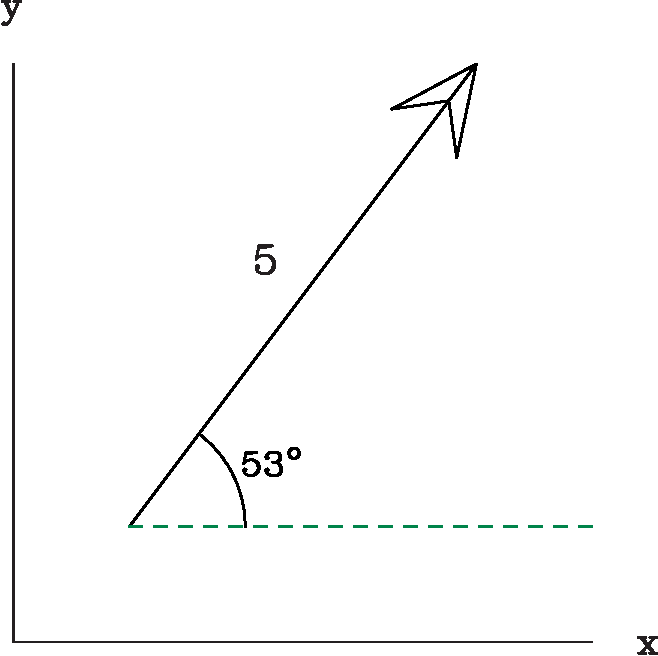
\includegraphics[width=0.7\textwidth]{vector-angle-crop.pdf}}
\Large
\centerline{Magnitude and direction}
\column{0.5\textwidth}
\centerline{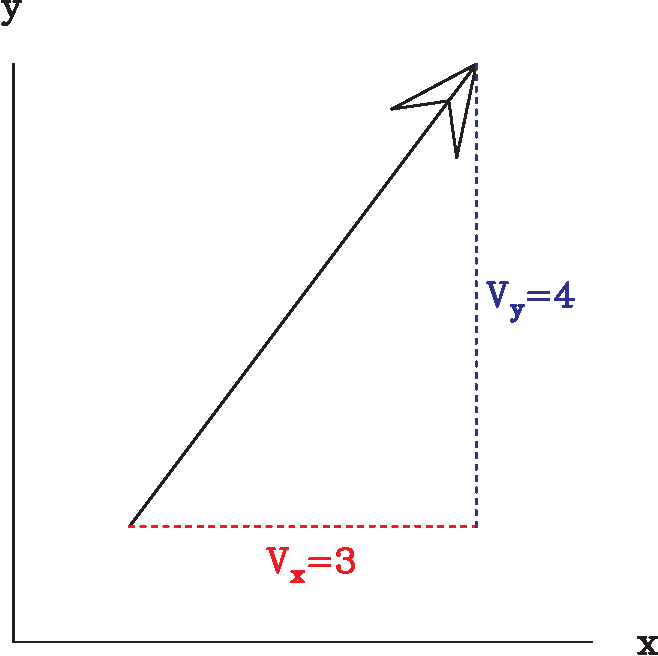
\includegraphics[width=0.7\textwidth]{vector-components-crop.pdf}}
\Large
\centerline{X and Y components}
\end{columns}
\bigskip
\bigskip
\Large
\centerline{How do we convert from one to the other?}
}


\frame{\frametitle{\textbf{How do we convert from one to the other?}}

\Huge

\color{A}A: Using algebra\\
\color{B}B: Using trigonometry\\
\color{C}C: Using calculus\\
\color{D}D: Using differential equations\\
}

\frame{\frametitle{\textbf{From magnitude and direction to components}}
	\begin{columns}
		\column{0.5\textwidth}
		\centerline{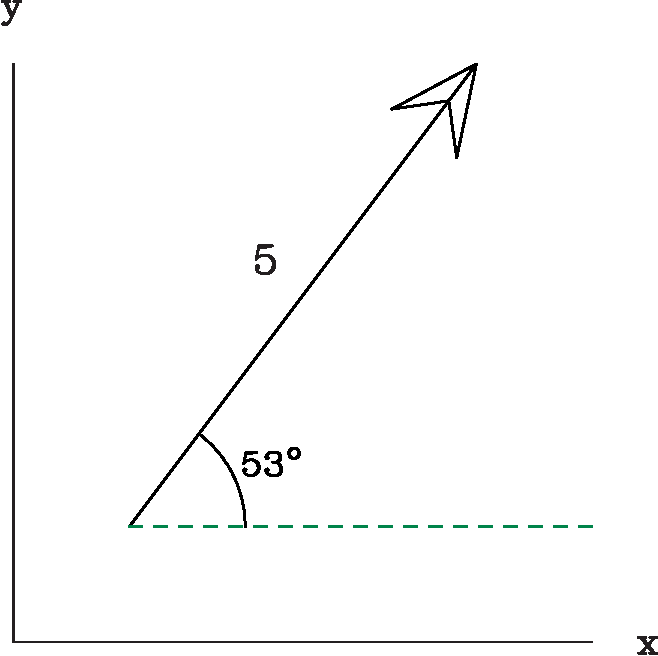
\includegraphics[width=0.7\textwidth]{vector-angle-crop.pdf}}
		\Large
		\centerline{Magnitude and direction}
		\column{0.5\textwidth}
		\large
		
		What is the $x-$component of this vector? \bigskip
		
		
		\color{A}A: $5 \cos 53^\circ$ \\
		\color{B}B: $5 \sin 53^\circ$ \\
		\color{C}C: $5 \tan 53^\circ$ \\
		\color{D}D: Something else
	
	\end{columns}

}

\frame{\frametitle{\textbf{From magnitude and direction to components}}
	\begin{columns}
		\column{0.5\textwidth}
		\centerline{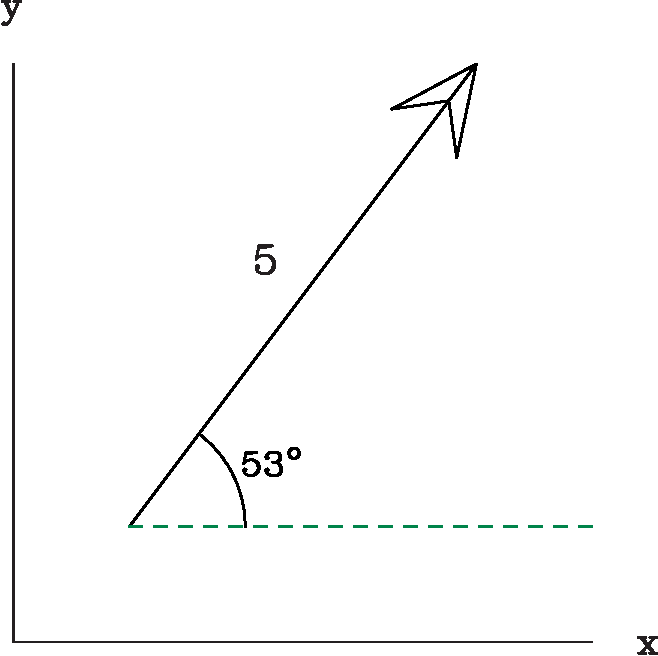
\includegraphics[width=0.7\textwidth]{vector-angle-crop.pdf}}
		\Large
		\centerline{Magnitude and direction}
		\column{0.5\textwidth}
		\large
		
		What is the $x-$component of this vector? \bigskip
		
		
		\color{A}A: $5 \cos 53^\circ$ \\
		\color{B}B: $5 \sin 53^\circ$ \\
		\color{C}C: $5 \tan 53^\circ$ \\
		\color{D}D: Something else
		
	\end{columns}
	
}



\frame{\frametitle{\textbf{From ``direction and magnitude'' to components}}
\centerline{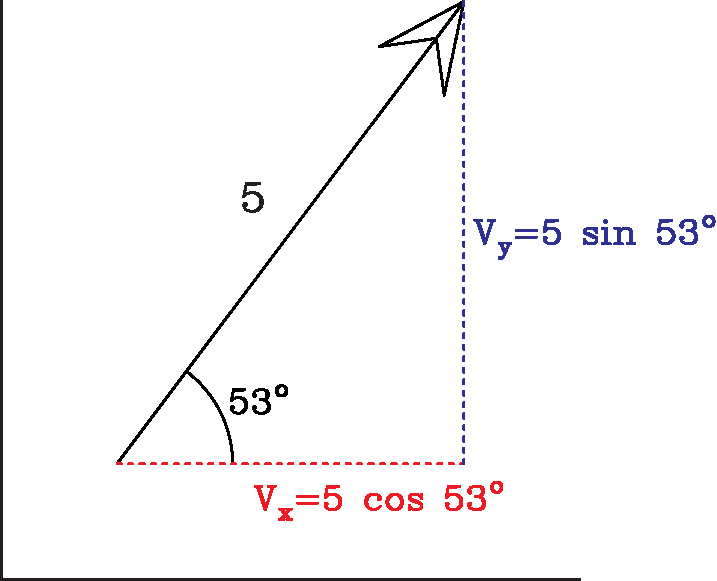
\includegraphics[width=0.6\textwidth]{vector-ang2comp-crop.pdf}}
}

\frame{\frametitle{\textbf{From components to direction and magnitude}}
\centerline{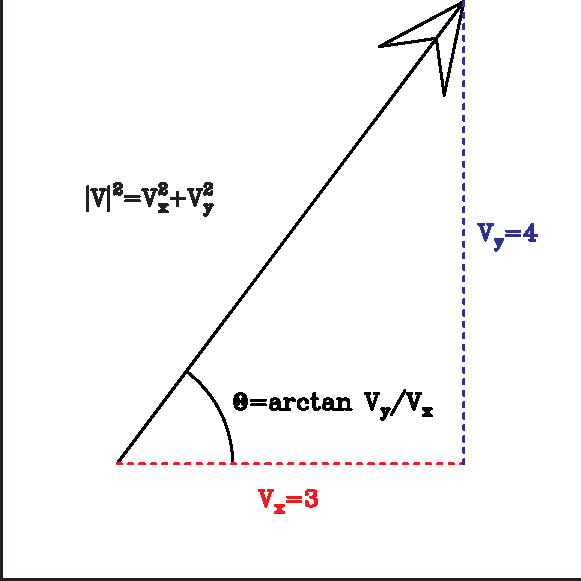
\includegraphics[width=0.6\textwidth]{vector-comp2ang-crop.pdf}}
}

\frame{

\Large


Suppose you have some vector $\vec A$ that you want to convert into components.
The $x$-component $A_x$ is:

\bigskip

\color{A}A: $A \cos \theta$\\
\color{B}B: $A \sin \theta$\\
\color{C}C: $A \tan \theta$\\
\color{D}D: $\frac{A}{\cos \theta}$\\
\color{E}E: It depends

}

\frame{\frametitle{\textbf{A warning!}}

\begin{center}\Large{You cannot memorize \\``$V \sin \theta$ is the $y$ component,  
\Large{$V \cos \theta$ is the $x$ component''!}} \end{center}
\bigskip
\bigskip
\centerline{\Large{This does {\it not} work in general; you have to actually draw the triangle.}}
}

\frame{\frametitle{\textbf{Adding vectors}}
We can also add vectors together by drawing them ``head to tail''. Here are two vectors:

\bigskip
\bigskip

\begin{columns}
\column{0.5\textwidth}
\centerline{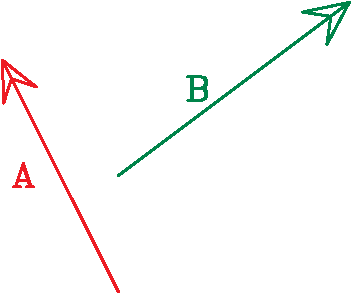
\includegraphics[width=0.6\textwidth]{vshow-crop.pdf}}
\column{0.5\textwidth}
\centerline{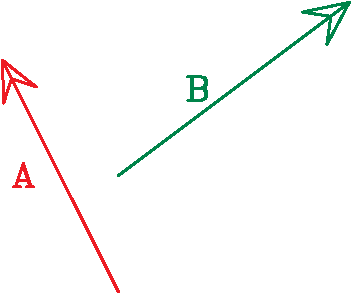
\includegraphics[width=0.6\textwidth]{vshow-crop.pdf}}
\end{columns}
}

\frame{
\centerline{\Large Does $\vec A + \vec B = \vec B + \vec A$?}

\bigskip
\bigskip
\bigskip

\Large

\BI
\item{A: Yes}
\item{B: No}
\EI

\pause

\bigskip
\bigskip
\bigskip

Yes: vector addition obeys the commutative property, just like ordinary addition
}

\frame{\frametitle{\textbf{Adding vectors}}
\centerline{We can also add vectors together by drawing them ``head to tail''. Here are two vectors:}

\bigskip
\bigskip

\begin{columns}
\column{0.5\textwidth}
\centerline{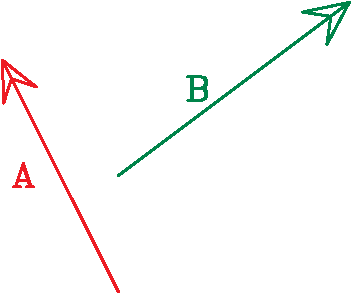
\includegraphics[width=0.6\textwidth]{vshow-crop.pdf}}
\column{0.5\textwidth}
\centerline{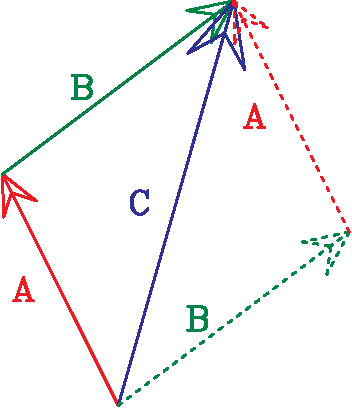
\includegraphics[width=0.6\textwidth]{vadd-crop.pdf}}
\end{columns}

\bigskip
\bigskip

\Large \centerline{$\color{Red}\vec A + \color{Green} \vec B = \color{Blue} \vec C$}

}

\frame{\frametitle{\textbf{Adding vectors: components}}
\centerline{\Large The component representation is much easier to work with!}

\Huge\centerline{$\color{Red}\vec A + \color{Green} \vec B = \color{Blue} \vec C \color{Black} \rightarrow {\color{Red} A_x + \color{Green} B_x = \color{Blue} C_x \choose \color{Red} A_y + \color{Green} B_y = \color{Blue} C_y}$}
}

\frame{\frametitle{\textbf{Adding vectors: components}}
\centerline{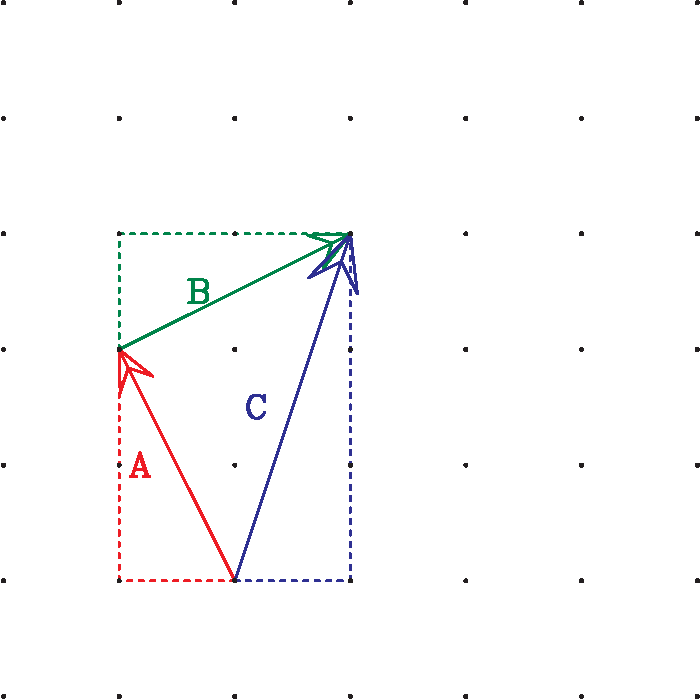
\includegraphics[width=0.4\textwidth]{vaddc-crop.pdf}}

\large
\bigskip

\centerline{To add two vectors, just add their components!}

\bigskip

\centerline{This is why it is almost always easiest to work in the component representation!}
}

\frame{\frametitle{\textbf{What does this do to our kinematics?}}
	\large Acceleration, velocity, and position relationships are still the same; they just apply {\color{Red}independently} for each component.

\normalsize
	
{\color{A}$\vec s$} is the position vector:
\begin{itemize}
	\item {{\color{A} $s_x$} or just {\color{A}$x$} is its $x$-component}
	\item {{\color{A} $s_y$} or just {\color{A}$y$} is its $y$-component}
\end{itemize}
\bigskip

{\color{B}$\vec v$} is the velocity vector:
\begin{itemize}
	\item {{\color{B} $v_x$} is its $x$-component}
	\item {{\color{B} $v_y$} is its $y$-component}
\end{itemize}
\bigskip

{\color{D}$\vec a$} is the acceleration vector:
\begin{itemize}
	\item {{\color{D} $a_x$} is its $x$-component}
	\item {{\color{D} $a_y$} is its $y$-component}
\end{itemize}


\bigskip

{\bf Do not get lazy} if you have multiple subscripts. For instance: {\color{C}$\vec v_0$} is the initial velocity vector:


\begin{itemize}
	\item {{\color{C} $v_{0,x}$} or {\color{C}${v_0}_x$} is its $x$-component}
	\item {{\color{C} $v_{0,y}$} or {\color{C}${v_0}_y$} is its $y$-component}
\end{itemize}

}


\frame{\frametitle{\textbf{What does this do to our kinematics?}}
\large Acceleration, velocity, and position relationships are still the same; they just apply {\color{Red}independently} for each component.
\Large



\begin{align*}
\vec v(t) =&\, \vec at + \vec v_0 \\
\vec s(t) =&\, \frac{1}{2}\vec a t^2 + \vec v_0 t + \vec s_0
\end{align*}

\pause

\begin{align*}
v_x(t) =&\, a_x t + v_{x,0} \\
v_y(t) =& a_y t + v_{y,0} \\
\end{align*}
\pause
\begin{align*}
x(t) =&\,  \frac{1}{2}  a_x t^2 + v_{x,0} t + x_0\\
\bigskip
y(t) =&\, \frac{1}{2}  a_y t^2 + v_{y,0} t + y_0
\end{align*}
}


\frame{
\centerline{\Large Which statement does {\it not} make sense?} 

\bigskip
\bigskip
\bigskip

\Large

\BI
\item{\color{A}A) $\vec A t = \vec B$}
\item{\color{B}B) $\vec A + \vec B + t = \vec C$}
\item{\color{C}C) $k(\vec A + \vec B) = k\vec A + k\vec B$}
\item{\color{D}D) $\vec A - \vec B = \vec C$}
\EI

\pause

\bigskip
\bigskip
\bigskip

B: You can't add a vector and a scalar. ``One mile north plus one inch'' -- which way is the inch?
}

\frame{\frametitle{\textbf{Problem solving: 2D kinematics, constant acceleration}}
\Large
\begin{enumerate}
\item{1. If you have vectors in the ``angle and magnitude'' form, convert them to components}
\bigskip

\item{2. Write down the kinematics relations, separately for $x$ and $y$}
\begin{itemize}
\large
\item{Many terms will usually be zero}
\item{Freefall: $a_x = 0$, $a_y = -g$ (with conventional choice of axes)}
\end{itemize}
\bigskip

\item{3. Understand what instant in time you want to know about}
\bigskip

\item{4. Put in what you know; solve for what you don't (using substitution, if necessary)}

\bigskip
\item{5. Convert vectors into whatever format you would like them in}
\end{enumerate}
\pause

\bigskip
\bigskip



\centerline{\Large{\color{Red}Every kinematics situation we will encounter can be done this way!}}
}

\frame{\frametitle{\textbf{Sample problems}}
\centerline{\Large{A rock is thrown at $v_0=10 m/s$ at $\theta=30^\circ$ above the horizontal.}}

\bigskip
\bigskip

\begin{itemize}
\large
\item{How far from its starting point is it after 2 seconds?}
\pause
\item{How far does it travel?}
\pause
\item{How high does it go?}
\pause
\item{What will its speed be when it strikes the ground?}
\end{itemize}
}


\frame{\frametitle{\textbf{We're done!}}
		
		\Large
		
		This is all of the material you will need for the first exam!
		
		\bigskip
		
		We have three recitations and two classes left; we're going to spend it practicing.
		
		\bigskip
		
		As with everything in physics, applying abstract ideas to the real world is the challenge. So we have set aside lots of time for it!


}


\end{document}
